\documentclass{article}
\usepackage{graphicx}
% \usepackage{array}
% \usepackage{multirow}
\usepackage{hyperref}
% \usepackage{booktabs}

\begin{document}

\title{Project 2}
\author{Jake Carlson}
\date{October 4, 2017}
\maketitle

\abstract
In this report, I will build several models to perform classification on federal payroll data. The years looked at are 2005 and 2013, years under the presidency of George W. Bush and Barack Obama respectively. I will perform data cleaning and preparation necessary to perform classification on this data set. Classification models used include artificial neural networks and random forests. We will see that under the Obama administration, pay was more closely related to the type of work an employee was doing, and employees with lower education levels were able to achieve higher levels of pay. Finally, I will present a model that allows potential employees to compare multiple job types and locations to see what combination could offer them the highest pay.
\newpage

\tableofcontents
\newpage

\section{Business Understanding}
In this project, I will again be analyzing the federal payroll data obtained by BuzzFeed News through the Freedom of Information Act. I will continue my analysis of the presidency of George W. Bush and Barack Obama by creating classification models based on the payroll data. Based on attributes of the employees, I will be trying to predict class labels such as the annual pay of the employee and what their level of education is. The various models will provide insight into how relevant each attribute is as predicitng the class label. For example, the heirarchy of splits in decision trees indicate what attributes are most relevant when determining the class label. By looking at how these models differ between the presidents, and how the ranking of attributes changes, we will gain insight into how each administration restructured the composition of the federal government.
\par
I will use a variety of classification models, including Decision Trees, Artificial Neural Networks, and Random Forests. I will compare the performance of these models to each other to see what models have the best performance in terms of both accuracy and the kappa score for classification on test data.

    \subsection{Annual Pay}
    By predicting Pay, we will see what attributes correspond to a higher pay rate. This would be useful for employees so that they can see what attributes they should look to change about themselves if they are looking to get a pay raise. For example, if Education has a strong relationship with higher pay rates, employees should consider pursuing higher education in order to recieve a raise.

    \subsection{Education Level}
    By predicting Education, we will be able to see what attributes are most related with having a higher or lower education level. If a particular agency is in need additional specialized labor, they could offer a subset of their employees financial aid to pursue higher education. This would allow that agency to promote from within, rather than looking for new employees.
    \par
    From Project 1 we determined that the vast majority of employees had either a high school diploma or a Bachelor's degree. This class imbalance will need to be addressed when creating classification models.\cite{proj1}

    \subsection{Career Planning}
    Finally, I will try to build the most accurrate model possible at predicting pay. I will use Age, Education, Station, SupervisoryStatus, and Category to train two models. Potentially, people could create new records for themselves and pass them through this model to see how much they would be paid if they decided to work at an agency in a particular state. I will create a record for myself and see what I would be able to expect if I got a job in the federal government.

\section{Data Preparation}
To prepare my data for classification, I reprocess the raw payroll data. I start by removing columns that I do not plan on using for classification. The attributes I save are given in Table \ref{tab:1}. I then replace unknown values with NA, make Pay a numeric attribute, pull out the encoding for what state the employee works in from Station, and create a column that holds the whole agency name for each employee. I join the four quarters for each of the four years I am looking at into one data frame, and save this frame to disk.
\par
When I load these data frames, I run some additional preparation to make sure the data is ready for classification and make sure the models will train as efficiently as possible. I create a region column which translates the state encoding in Station to the actual name of the state. I convert Pay to an ordinal variable from a continuous variable by descretizing into six classes. The Pay groups are given in Table \ref{tab:2}. I then convert the ordinal Age variable to a ratio variable by taking the middle of the age range for each occurance The Age translation is given in Table \ref{tab:3}. I break Education up into groups by what level of education the employee achieved. The groups I used are listed in Table \ref{tab:9}. Next I convert the ordinal Length of Service variable to a ratio varible by taking the middle of the time span for each occurance. The translation for LOS is given in Table \ref{tab:4}. My preparation function also allows for a subset of agencies to be choosen from the saved data files.
\par
The scale and range of all of the attributes in the final data set are given in Table \ref{tab:5}. When I go to create a model based on a subset of my choosen columns, I will throw out any entries that are incomplete. The count of the number of records that are complete, as well as the percentage of records that are complete for each year are given in Table \ref{tab:6}.

    \begin{center}
        \begin{table}
            \centering
            \begin{tabular}{ |c|c|c| }
                \hline
                Attribute & Scale & Description \\
                \hline
                Agency & Categorical & The four character encoding for the agency the employee worked at. \\
                Station & Categorical & The state the employee works in. \\
                Age & Ordinal & The age range of the employee, given in 5 year intervals. \\
                Education & Ordinal & The education level achieved by the employee. \\
                LOS & Ordinal & The number of years the employee has worked in the federal governemnt, given in 5 year intervals. \\
                Category & Categorical & The general type of work the employee does, following the PATCO acronym. \\
                Pay & Ratio & The annual pay the employee receives in U.S. Dollars. \\
                SupervisoryStatus & Categorical & The level of leadership the employee has achieved. \\
                \hline
            \end{tabular}
            \caption{Attributes To Be Used For Classification}
            \label{tab:1}
        \end{table}
    \end{center}

    \begin{center}
        \begin{table}
            \centering
            \begin{tabular}{ |c| }
                \hline
                Pay Ranges \\
                \hline
                $<$30k \\
                30-50k \\
                50-70k \\
                70-90k \\
                90-110k \\
                $>$110k \\
                \hline
            \end{tabular}
            \caption{The Pay Ranges Used To Descretize Pay}
            \label{tab:2}
        \end{table}
    \end{center}

    \begin{center}
        \begin{table}
            \centering
            \begin{tabular}{ |c|c| }
                \hline
                Age Range & Ratio Value \\
                \hline
                15-19 & 17 \\
                20-24 & 22 \\
                25-29 & 27 \\
                30-34 & 32 \\
                35-39 & 37 \\
                40-44 & 42 \\
                45-49 & 47 \\
                50-54 & 52 \\
                55-59 & 57 \\
                60-64 & 62 \\
                65-69 & 67 \\
                70-74 & 72 \\
                75+ & 75 \\
                \hline
            \end{tabular}
            \caption{Original Age Ranges In Years And The Choosen Value For Classification}
            \label{tab:3}
        \end{table}
    \end{center}

    \begin{center}
        \begin{table}
            \centering
            \begin{tabular}{ |c|c|c| }
                \hline
                Group & Education Levels & Description \\
                \hline
                Elm & 0, 1 & Reached or completed elementary school \\
                HS & 3, 4, 5, 6 & Reached or completed high school or an occupational program \\
                Col & 7, 8, 9, 10, 11, 12, 13 & Reached or completed college with a Bachelor's degree \\
                Grad & 14, 15, 16, 17, 18, 19, 20 & Any level of graduate studies, excluding a Doctorate \\
                Doc & 21, 22 & A Doctorate or Post-Doctorate degree \\
                \hline
            \end{tabular}
            \caption{Ordinal Education Groups}
            \label{tab:9}
        \end{table}
    \end{center}

    \begin{center}
        \begin{table}
            \centering
            \begin{tabular}{ |c|c| }
                \hline
                LOS Range & Ratio Value \\
                \hline
                $<$ 1 & 1 \\
                1-2 & 1 \\
                3-4 & 3 \\
                5-9 & 7 \\
                10-14 & 12 \\
                15-19 & 17 \\
                20-24 & 22 \\
                25-29 & 27 \\
                30-34 & 32 \\
                35+ & 35 \\
                \hline
            \end{tabular}
            \caption{Original Length Of Service Ranges And The Choosen Value For Classification}
            \label{tab:4}
        \end{table}
    \end{center}

    \begin{center}
        \begin{table}
            \centering
            \begin{tabular}{ |c|c|c| }
                \hline
                Attribute & Scale & Range \\
                \hline
                Agency & Nominal & Unique four characters for each agency \\
                Station & Nominal & 1-56, some values missing \\
                Age & Ratio & 17-72 by 5, 75 \\
                Education & Ordinal & Elm, HS, Col, Grad, Doc \\
                LOS & Ratio & 1, 3, 7-32 by 5, 35 \\
                Category & Nominal & P, A, T, C, O, B \\
                Pay & Ordinal & $<$30k, 30-50k, 50-70k, 70-90k, 90-110k, $>$110k \\
                SupervisoryStatus & Categorical & 2, 4, 5, 6, 7, 8 \\
                \hline
            \end{tabular}
            \caption{Final Data Set Attributes}
            \label{tab:5}
        \end{table}
    \end{center}

    \begin{center}
        \begin{table}
            \centering
            \begin{tabular}{ |c|c|c| }
                \hline
                Year & Number Complete & Percentage of Original \\
                \hline
                2001 & 2,535,278 & 58.09\% \\
                2005 & 2,598,800 & 55.05\% \\
                2009 & 2,862,972 & 55.22\% \\
                2013 & 3,136,697 & 58.91\% \\
                \hline
            \end{tabular}
            \caption{The Number Of Complete Records For Each Year}
            \label{tab:6}
        \end{table}
    \end{center}

\section{Modeling}
Next I will begin creating models for the each of the cases outlined in the Business Understanding. I will create two models for each of the cases and compare their performance using 10-fold cross validation. I will identify the model that perfoms the best. I will show the structure of the model if possible and see how these structures change with the presidency. To make training and evaluation easier, I will create a pipeline to break up the data, train the models, test them, and return the results.

    \subsection{Annual Pay}
    I will be modeling Pay for the Department of Justice. I will compare the performance of decision trees and random forests. In order to speed up the training of my models, I only want to pass in the attributes that are most important for predicting Pay. To determine these attributes I examine the results of both cfs, which uses correlation and cross entropy, and consistency, which uses a consistency measure, to determine variable importance. The most important attributes given by consistency in descending order are Age, Education, Length of Service, Category, and SupervisoryStatus. The most important measures by cfs are Education and Category. I will use Age, Education, and Category for training my models because, based on these rankings, I think these are the most relevant attributes.
    \par
    The accuracy and kappa scores for each of the models is given in Table \ref{tab:7}. These scores are not great, but the random forests consistently beat out the decision tree. The most important variables given by the random forests are Education and Age followed by whether or not the employee is in a technical role or a clerical role. The decision tree concurs with the random forests that Education is the most important attribute, followed by whether the employee is in a techinical role or not. This indicates that the education is strongly related with how much an employee makes in the Department of Justice.
    \par
    The structure of the decision tree given in Figure \ref{paydesctree2005} shows that clerical roles tend to be paid less and technical roles tend to be paid more. I want to see how these models change under the Obama administration, so I will rerun these using the 2013 data set. Again, Education is the most important attribute for both the decision tree and the random forest, followed by Age. The structure of the decision tree for 2013 is given in Figure \ref{paydesctree2013}. We see that the splits in the decision tree closest to the root have to do with what Category an employee is in. The difference in the complexity of the decision tree would appear to indicate that, under the Obama administration, pay was more closely related to what type of position you held.

    \begin{center}
        \begin{table}
            \centering
            \begin{tabular}{ |c|c|c|c|c|c|c|c| }
                \hline
                & Accuracy \\
                \hline
                Classifier & Min. & 1st Qu. & Median & Mean & 3rd Qu. & Max. & NA's \\
                Decision Trees & 0.5176392 & 0.5211121 & 0.5275774 & 0.5289369 & 0.5376409 & 0.5415454 & 0 \\
                Random Forests & 0.5619261 & 0.5658214 & 0.5704048 & 0.5698463 & 0.5739125 & 0.5764363 & 0 \\
                \hline
                & Kappa \\
                \hline
                Classifier & Min. & 1st Qu. & Median & Mean & 3rd Qu. & Max. & NA's \\
                Decision Trees & 0.3466076 & 0.3497777 & 0.3672808 & 0.3688381 & 0.3881202 & 0.3946472 & 0 \\
                Random Forests & 0.4274982 & 0.4319667 & 0.4382973 & 0.4374711 & 0.4428353 & 0.4456237 & 0 \\
                \hline
            \end{tabular}
            \caption{The Accuracy And Kappa Score for Decision Trees and Random Forests}
            \label{tab:7}
        \end{table}
    \end{center}

    \begin{center}
        \begin{table}
            \centering
            \begin{tabular}{ |c|c|c|c|c| }
                \hline
                % & \multicomlum{2}{|c|}{2005} & \multicomlum{2}{|c|}{2013} \\
                & 2005 & 2005 & 2013 & 2013 \\
                \hline
                Decision Tree & Education & 9932.9 & Education & 9382.2 \\
                & CategoryT & 7682.5 & Age & 7867.3 \\
                & CategoryP & 5599.9 & CategoryP & 5382.3 \\
                & CategotyC & 5305.0 & CategoryB & 4715.5 \\
                \hline
                Random Forest & Education & 10345.0 & Education & 11113.4 \\
                & Age & 4089.5 & Age & 5470.7 \\
                & CategoryT & 2805.7 & CategoryC & 1601.5 \\
                & CategoryC & 2393.5 & CategoryT & 1476.4 \\
                \hline
            \end{tabular}
            \caption{Variable Importance Rankings for Predicting Pay for Decision Trees and Random Forests in 2005 and 2013}
            \label{tab:8}
        \end{table}
    \end{center}

    \begin{center}
        \begin{figure}
            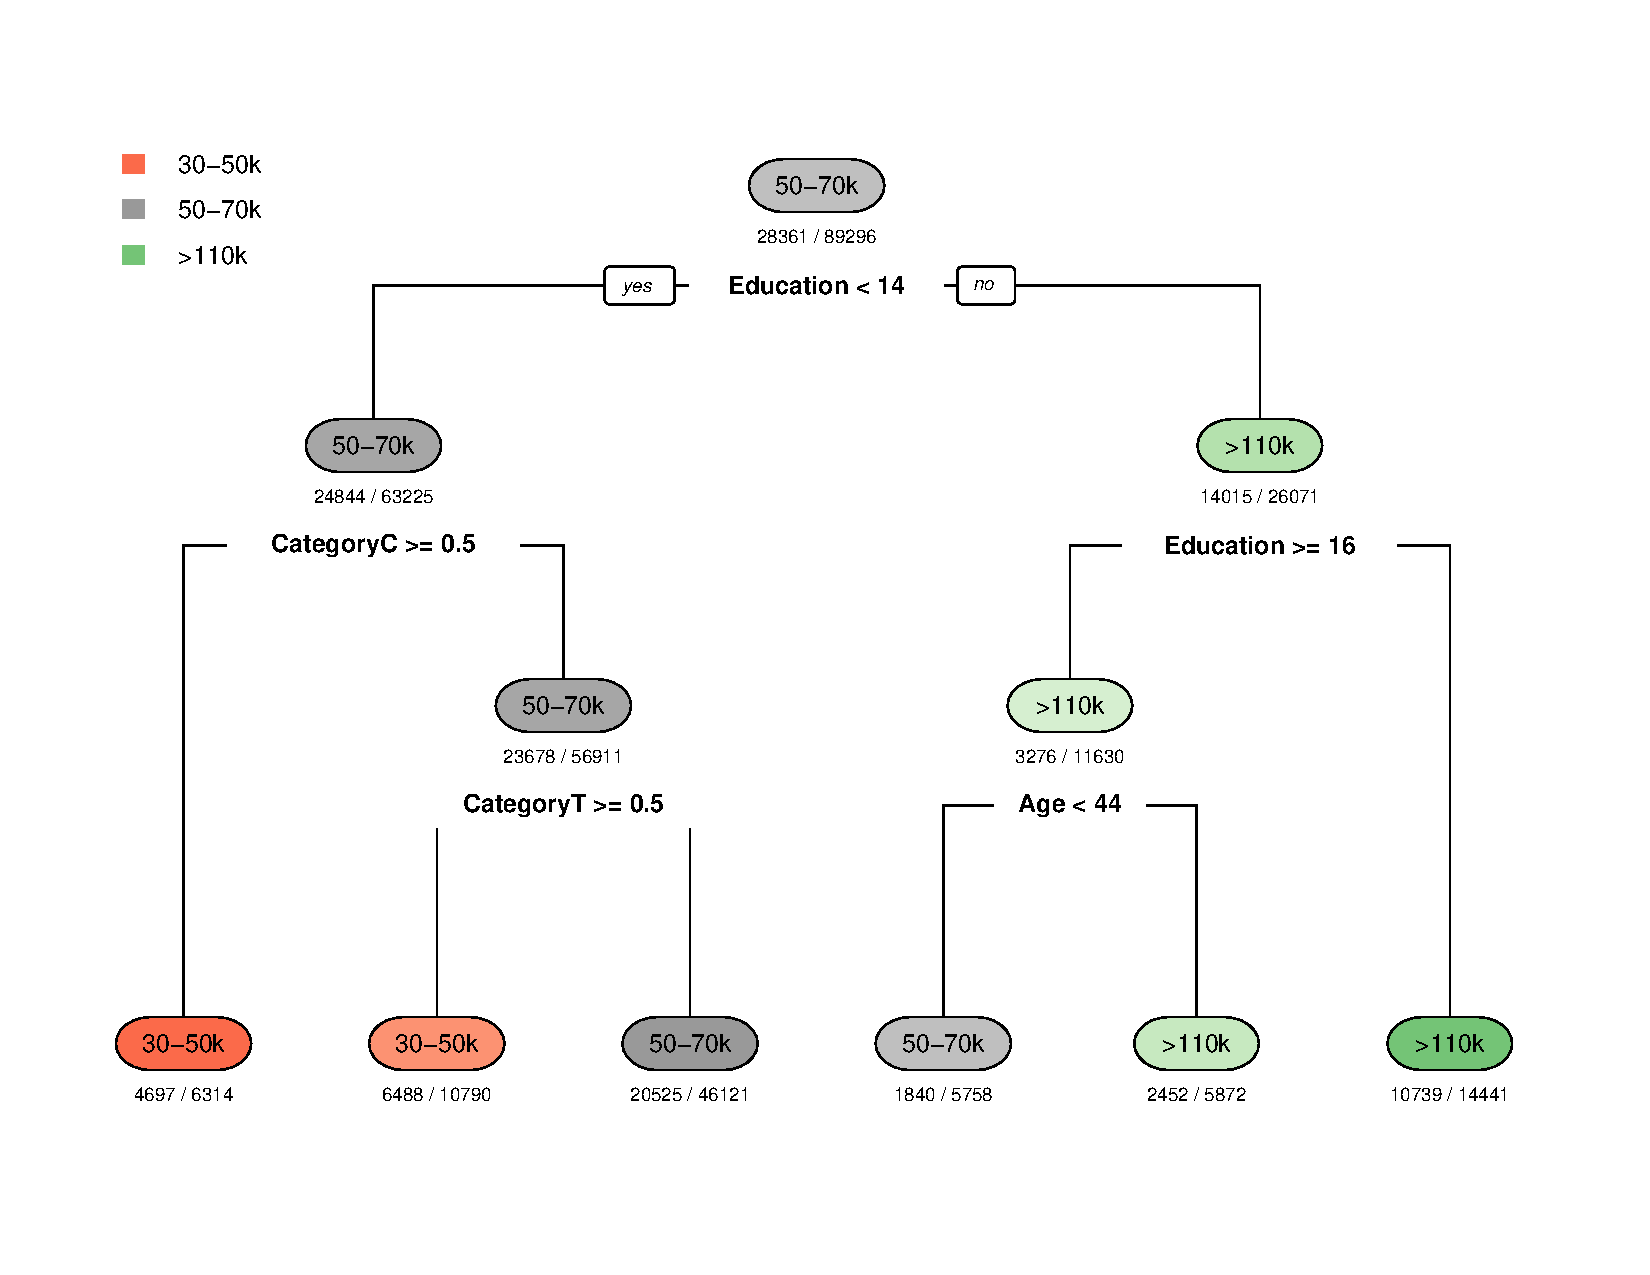
\includegraphics[scale=0.4]{./images/pay-decision-tree-2005.pdf}
            \caption{The Structue of the Decision Tree for Pay in the Department of Justice in 2005}
            \label{paydesctree2005}
        \end{figure}
    \end{center}

    \begin{center}
        \begin{figure}
            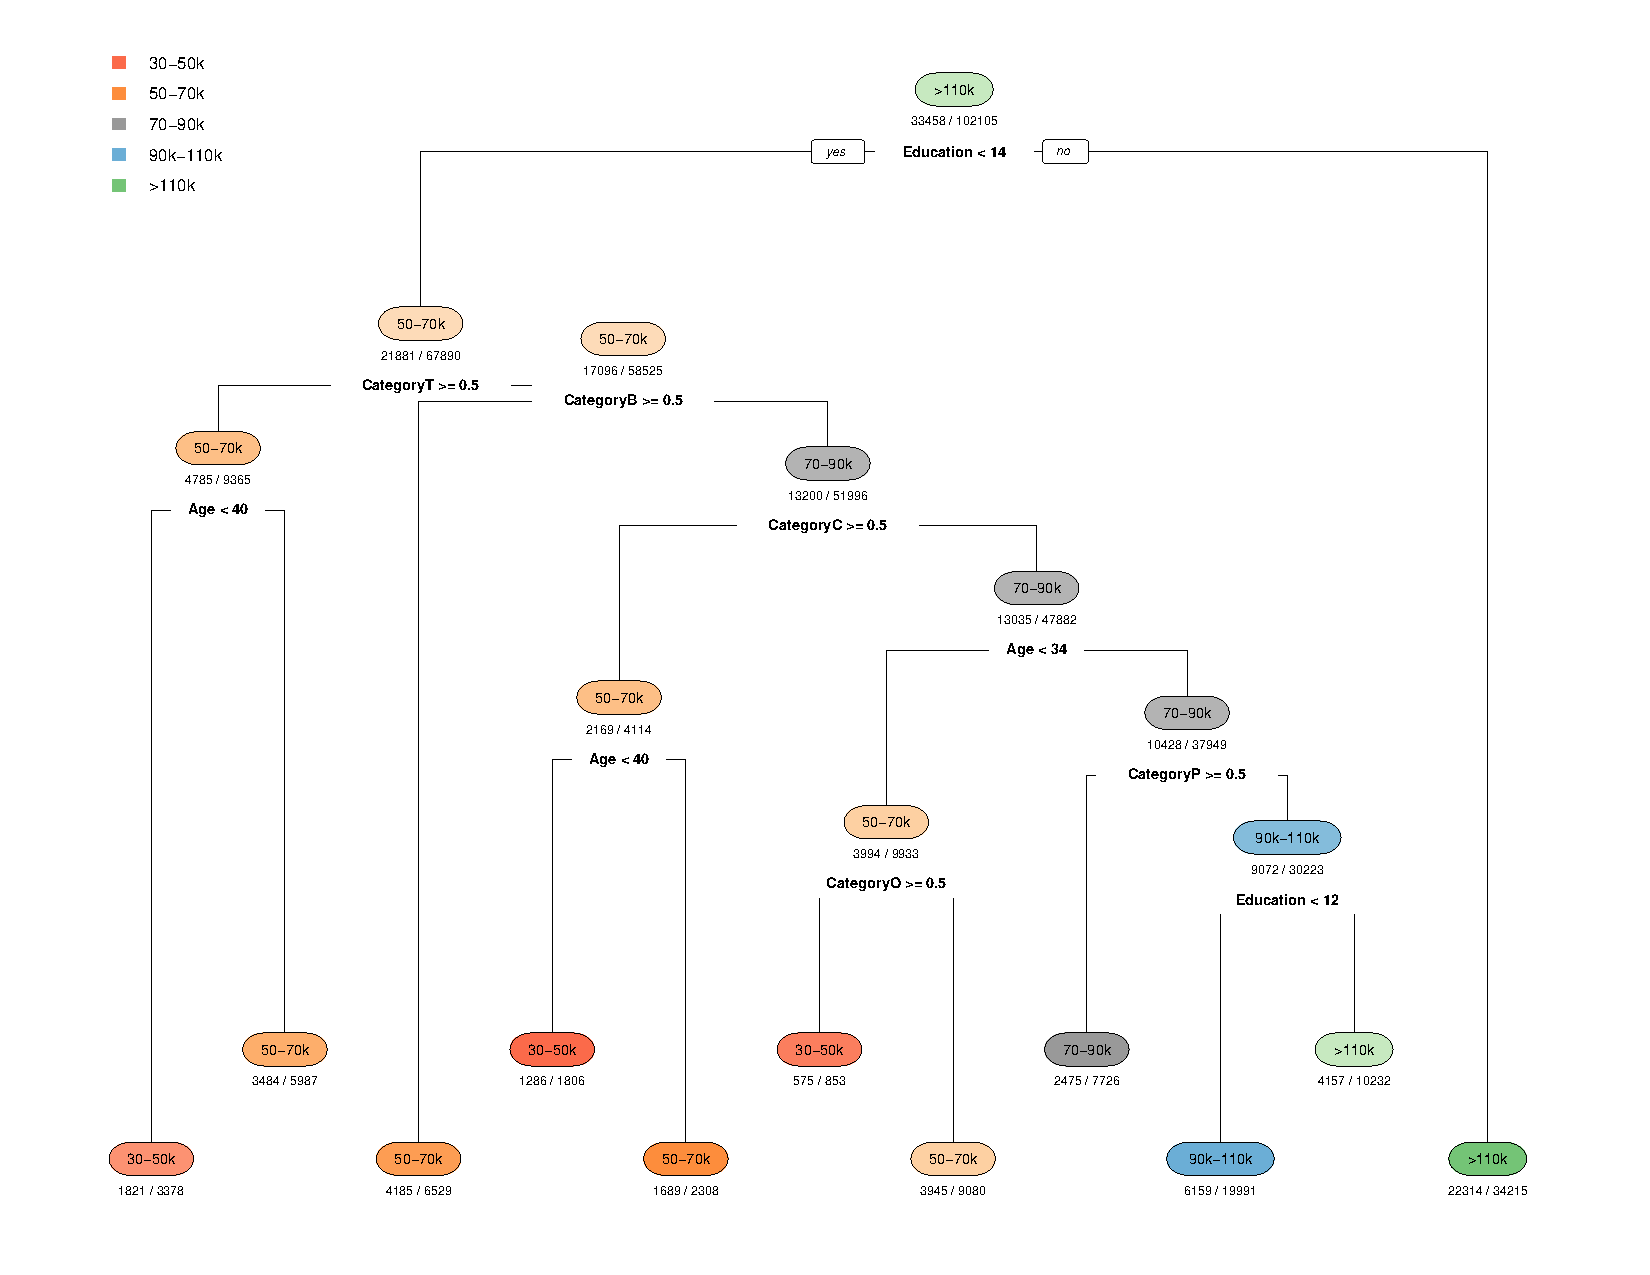
\includegraphics[scale=0.4]{./images/pay-decision-tree-2013.pdf}
            \caption{The Structue of the Decision Tree for Pay in the Department of Justice in 2013}
            \label{paydesctree2013}
        \end{figure}
    \end{center}

    \subsection{Education Level}
    I will model Education for the Department of Justice again using decision trees and random forests. The models for Pay showed that the Category and Education are the most relevant attributes for predicting the Pay of an employee. I would expect Category to be an important attribute in predicting Education. I will again use cfs and consistency to determine the most relevant attributes to use when training my models for Education. Consistency gives the most important attributes as Age, Length of Service, Category, and SupervisoryStatus. Cfs gives the most important attributes as Category, and Pay. I will use Age, Category, and Pay to build my models.
    \par
    The models had comparable accuracy and kappa scores to the scores in Table \ref{tab:7}. Again, the random forest consistently beat the decision tree with a maximum accuracy of 0.616 over 0.604 and a maximum kappa of 0.415 over 0.399. The most important attributes for 2005 and 2013 are given in Table \ref{tab:10}. I have also provided the decision tree structure for 2005 in Figure \ref{edudesctree2005} and 2013 in Figure \ref{edudesctree2013}.
    \par
    It is interesting how similar the structures of the trees are. The trees are identical except for the last split between college and graduate education levels. The relationship between reaching graduate studies and having a pay greater than 100k. The most accurate class in both decision trees is where the employee reached graduate level studies and has an annual income greater than 100k. The accuracy of this class actually drops moving from Bush to Obama, indicating employees with lower levels of education were able to reach a higher pay grade.

    \begin{center}
        \begin{table}
            \centering
            \begin{tabular}{ |c|c|c|c|c| }
                \hline
                & 2005 & 2005 & 2013 & 2013 \\
                \hline
                Decision Tree & Pay.110k & 11733.8 & Pay.110k & 11483.9 \\
                & CategoryP & 9518.1 & CategoryP & 10257.4 \\
                & Pay30.50k & 3680.3 & Pay50.70k & 5405.1 \\
                & CategoryB & 2814.5 & CategoryB & 3793.9 \\
                \hline
                Random Forest & CategoryP & 9515.0 & CategoryP & 10257.5 \\
                & Pay.110k & 3171.8 & Pay.110k & 3554.9 \\
                & Age & 930.5 & CategoryB & 1421.8 \\
                & CategoryB & 915.6 & Age & 1384.9 \\
                \hline
            \end{tabular}
            \caption{Variable Importance Rankings for Predicting Education for Decision Trees and Random Forests in 2005 and 2013}
            \label{tab:10}
        \end{table}
    \end{center}

    \begin{center}
        \begin{figure}
            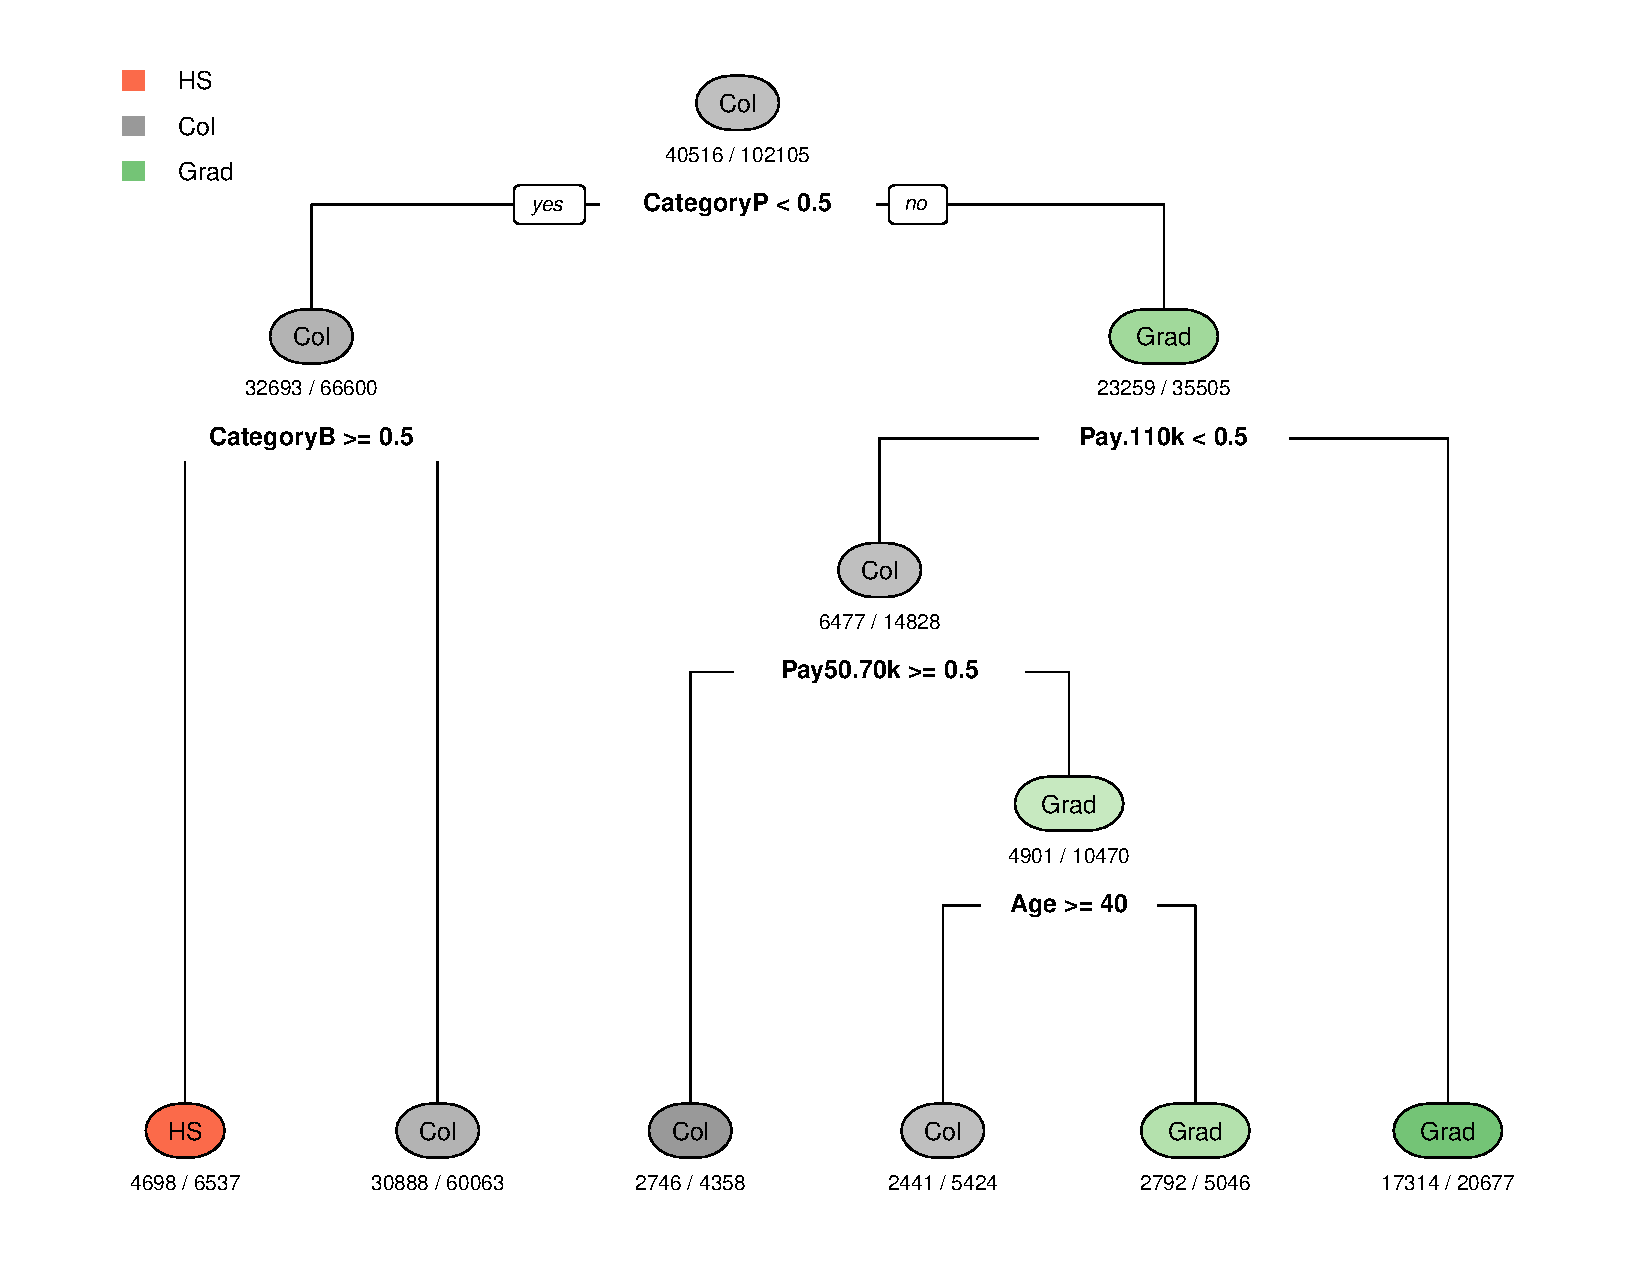
\includegraphics[scale=0.4]{./images/edu-decision-tree-2013.pdf}
            \caption{The Structue of the Decision Tree for Education in the Department of Justice in 2013}
            \label{edudesctree2013}
        \end{figure}
    \end{center}

    \begin{center}
        \begin{figure}
            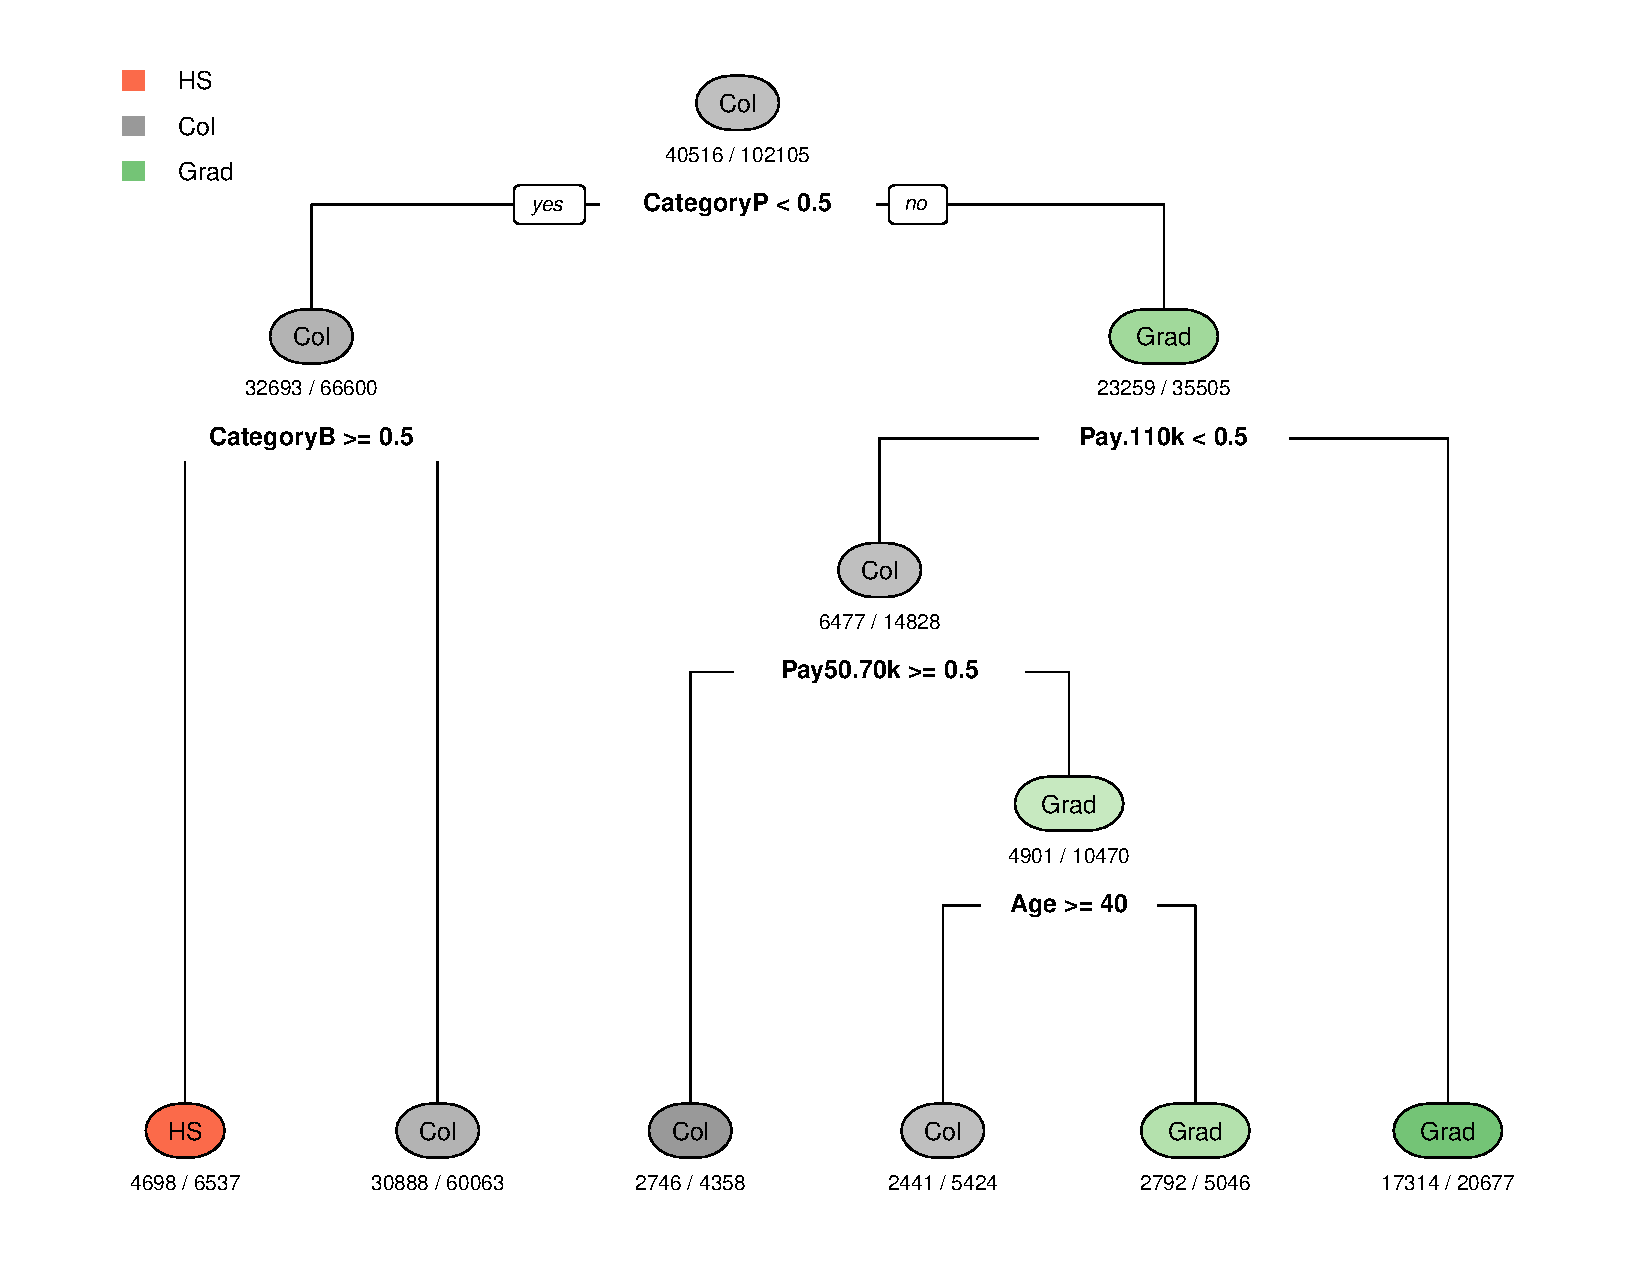
\includegraphics[scale=0.4]{./images/edu-decision-tree-2013.pdf}
            \caption{The Structue of the Decision Tree for Education in the Department of Justice in 2013}
            \label{edudesctree2013}
        \end{figure}
    \end{center}

    \subsection{Career Planning}
    Next I will compare the accuracy of linear support vector machines and artificial neural networks to see which model would be most useful for predicting the Pay of a potential new employee. If I were to work in the federal government, I would be most interested in working at NASA. For these models, I will train on the 2013 data for NASA based off of the attributes new employees would know about themselves. These attributes are Age, Education, Category, and the state they want to work in.
    \par
    To start this section I will train models on the raw data to see how well they do. I am not accounting for the Pay class imbalance at this point. The distribution of Pay for this data set is given in Table \ref{tab:11}. We see that neural networks out-perform support vector machines consistently. These are also much better scores than we saw for decision trees or random forests, although the data set has changed. The resulting scores are in Table \ref{tab:12}
    \par
    I will see if it is possible to boost these scores anymore by balancing the data sets. I will remove the $<$30k class because of how few instances there are, and I will sample 16,000 instances of the remaining classes. The accuracy and kappa scores for these classifiers are given in Table \ref{tab:13}. We see that balancing the data in this fashion produces lower accuracy scores. The maximum accuracy on balanced data for both neural networks and support vector machines are lower than the minimum accuracy on the unbalanced data.
    \par
    I will use the model with the highest accuracy to predict what my pay would be at NASA. I am planning on completing a Master's degree before entering the workforce, and I am looking for a professional role. The attributes of my record are given in Table \ref{tab:14}. I am open to working in both Texas and California, so I will create records for each of these circumstances and compare the outputs.
    \par
    My model predicts that I would make between \$90,000 and \$110,000 in both California and Texas. There is a problem with the input fields. It appears all of the entries for employees in California and a few other states were removed. The station was marked NA even though the specific agency was known. In order to resolve this, I would need to incorporate additional data that maps subgroups of NASA to the state those groups are located. This would allow me to maintain more of the entries, and could possibly increase the accuracy of my classifier. With this in mind, the values predicted approximate the national average pay for people with the attributes I presented at NASA.

    \begin{center}
        \begin{table}
            \centering
            \begin{tabular}{ |c|c| }
                \hline
                Pay & Count \\
                \hline
                $<$30k & 52 \\
                30-50k & 1,809 \\
                50-70k & 4,158 \\
                70-90k & 8,743 \\
                90-110k & 16,742 \\
                $>$110k & 40,431 \\
                \hline
            \end{tabular}
            \caption{Count for Each Pay Group at NASA in 2013}
            \label{tab:11}
        \end{table}
    \end{center}

    \begin{center}
        \begin{table}
            \centering
            \begin{tabular}{ |c|c|c|c|c|c|c|c| }
                \hline
                & Accuracy \\
                \hline
                Classifier & Min. & 1st Qu. & Median & Mean & 3rd Qu. & Max. & NA's \\
                SVMs & 0.6601880 & 0.6644062 & 0.6725758 & 0.6713937 & 0.6760624 & 0.6859645 & 0 \\
                Neural Networks & 0.5637412 & 0.6704036 & 0.6762093 & 0.6678942 & 0.6879576 & 0.6941478 & 0 \\
                \hline
                & Kappa \\
                \hline
                Classifier & Min. & 1st Qu. & Median & Mean & 3rd Qu. & Max. & NA's \\
                SVMs & 0.4070017 & 0.4118411 & 0.4201859 & 0.4240386 & 0.4333163 & 0.4546614 & 0 \\
                Neural Networks & 0.0000000 & 0.4182674 & 0.4355880 & 0.3938948 & 0.4567227 & 0.4630322 & 0 \\
                \hline
            \end{tabular}
            \caption{The Accuracy And Kappa Score for Support Vector Machines and Artificial Neural Networks}
            \label{tab:12}
        \end{table}
    \end{center}

    \begin{center}
        \begin{table}
            \centering
            \begin{tabular}{ |c|c|c|c|c|c|c|c| }
                \hline
                & Accuracy \\
                \hline
                Classifier & Min. & 1st Qu. & Median & Mean & 3rd Qu. & Max. & NA's \\
                SVMs & 0.5493379 & 0.5561194 & 0.5596496 & 0.5607548 & 0.5653801 & 0.5742046 & 0 \\
                Neural Networks & 0.4730884 & 0.5043785 & 0.5175654 & 0.5169082 & 0.5317104 & 0.5614185 & 0 \\
                \hline
                & Kappa \\
                \hline
                Classifier & Min. & 1st Qu. & Median & Mean & 3rd Qu. & Max. & NA's \\
                SVMs & 0.3975886 & 0.4006295 & 0.4063126 & 0.4078579 & 0.4127812 & 0.4235146 & 0 \\
                Neural Networks & 0.3049110 & 0.3453421 & 0.3532155 & 0.3552601 & 0.3684754 & 0.3994109 & 0 \\
                \hline
            \end{tabular}
            \caption{The Accuracy And Kappa Score for Support Vector Machines and Artificial Neural Networks with Balanced Data}
            \label{tab:13}
        \end{table}
    \end{center}

    \begin{center}
        \begin{table}
            \centering
            \begin{tabular}{ |c|c|c|c|c| }
                \hline
                Age & Education & region & Category & Predicted Pay \\
                \hline
                22 & Grad & Texas & P & 90-110k \\
                22 & Grad & California & P & 90-110k \\
                \hline
            \end{tabular}
            \caption{Trial Record for Author}
            \label{tab:14}
        \end{table}
    \end{center}

\section{Evaluation and Deployment}
Next I will asses how useful these models would be to the stake holders outlined in the Business Understanding section.

    \subsection{Annual Pay}
    Initially, I thought employees could use the models generated to predict annual pay to see what attributes would contribute most to an increase in pay. Based off the structure of the decision trees, for lower pay ranges, the best option would be to change the type of work the employee does. This is not an easy option for most employees. For higher incomes, the way to achieve a higher pay is to either achieve a higher level of education, or grow older. Again, neither of these are particularly useful, so these models would not provide much value to employees.

    \subsection{Education}
    For Education, an agency could potentially identify employees who would take advantage of financial aid to improve their education. These employees would be able to perform more specialized labor. If the Department of Justice is looking for more clerical or techinical type employees, blue collar employees would be a good target for this type of program. The agency would have to offer money to encourage these employees to enroll in college classes. If the department needs more employees with Graduate level education, College educated employees making more than 50-70k a year would be a good target for this type of program. However, these employees could likely pay for the higher education themselves and would not need assistance from the agency.
    \par
    This model would serve useful for making this distinction between employees.

    \subsection{Career Planning}
    For this section, potential employees could use this model to determine what state or job category would potentially offer them the highest pay. Unfortunately, because I threw out incomplete rows, this model would not be useful unless the people using it are trying to decide between states that were represented in the training data. Because I was looking at California and Texas, this model does not do much for me. It would be more useful to look at the national average pay.

\begin{thebibliography}{10}
    \bibitem{proj1}
    Jake Carlson
    \textit{CSE 5331 - Data Mining Project 1}
    \texttt{https://github.com/jakecarlson1/data-mining-projects/blob/master/}
    \texttt{project-1/report/carlson-project-1.pdf}

\end{thebibliography}

\end{document}
